\PassOptionsToPackage{dvipsnames, table}{xcolor}
\documentclass[dvipsnames, table, 11pt]{article}

\textwidth=7in
\textheight=9.5in
\hoffset=-1in
\voffset=-1in
\parskip=10pt
\parindent=0pt

\usepackage{style}

\begin{document}

\section{Anthology/Geneaology of early-warning signals}\label{sec:literature_review}
The theory of early-warning signals of critical transitions was motivated by applications in climate science and ecology.
Since the mid 2000s the need to quantify and predict catastrophic tipping points in ecosystems led to a number of empircal indicators being proposed.
While not exhaustive, what follows is a brief review of the existing literature of the field.

\subsection{Early developments}
The loss of resilience of ecosystems in recovering from external perturbations (such as lakes etc...) was initially noted to be captured by an increase in the variance of the species' population \cite{Carpenter2006, VanNes2007}.

\begin{figure}[H]
    \centering 
    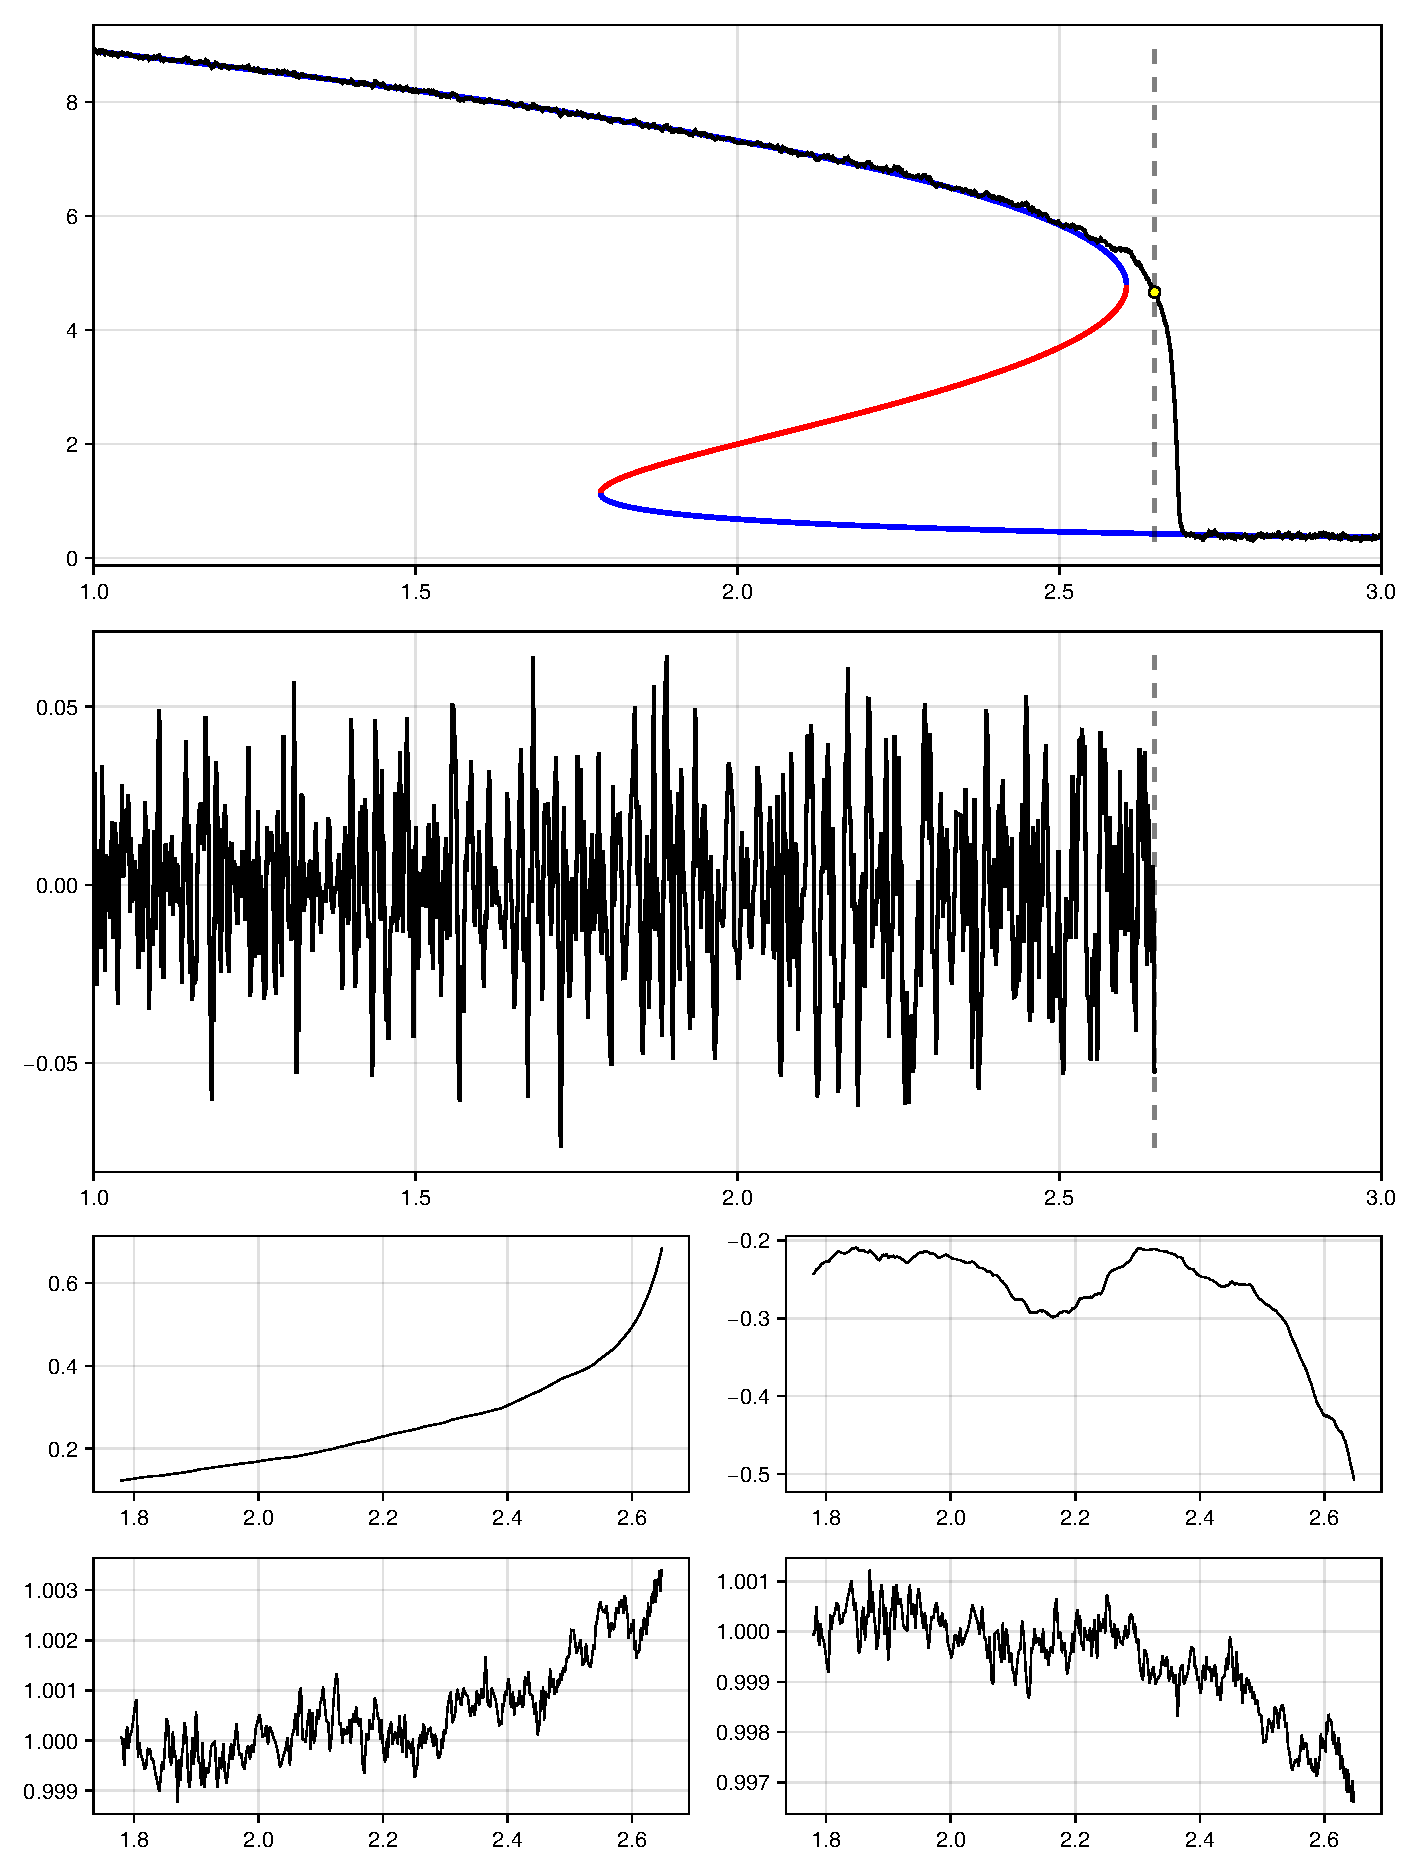
\includegraphics[keepaspectratio, width=\textwidth]{./figures/traditional_ews_comparison.pdf}
    \caption{Most used early-warning signals applied to a slowly ramped harvested population model following a bistable saddle-node bifurcation.}
    \label{fig:traditional_ews_comparison}
\end{figure}

Shortly after the same property was linked to similar types of catastrophic transitions in changing climates \cite{Dakos2008}.
In both cases this loss of resilience was associated to a phenomenon known in dynamical systems and statistical mechanics as \textit{critical slowing down} (CSD).
In these early works the authors argued that a complex system evolving over time and in a state of equilibrium should, if stochastically perturbed, show slower recovery rates as the attracting state weakens.
This slower return to equilibrium should result in an increase in variance and autocorrelation of the timeseries of the state due to loss of resilience by the system in absorbing perturbations.
Later on it was noted that, in bi- or multi-stable systems, the presence of alternative attractors naturally distorts any symmetry in the basin of attraction of the observed state which entails that an increase in the asymmetry of the timeseries should be registered as the basin of attractions shrinks.
Such behaviour would thus ideally be captured by an increase or decrease in the skewness of the timeseries \cite{Guttal2008}.

\subsection{Reviews, comparisons and performance/robustness/statistical significance}
With increasing interest towards the problem more and more indicators had been proposed. 
Eventually a review of the state of the art was published in 2009 \cite{Scheffer2009} by some of the major contributors thus far. 
In this work it was suggested that generic early-warning signals should exist for a variety of collapses in complex systems.
A subsequent paper \cite{Dakos2012} compared the performace of these generic indicators on a dataset of two synthetic timeseries of a bi-stable, biomass collapse subject to increasing harvesting.
Leading indicators were thereby grouped into \textit{metric-based}, meant to capture characteristic changes of timeseries data with no a-priori knowledge of the model generating it, and \textit{model-based}, which conversely attempted to fit some model parameters in order to infere incoming tipping points. 
In the same year a similar comparison \cite{Lenton2012} addressed the issue of robustness of detected signals when applied to paleoclimate records of ancient climate trasitions as well as complicated ocean model experiments. 

\subsection{Extension to high-dimensional systems}
While the initial efforts of detecting tipping points have focused on univariate timeseries in low-dimensions, the emphasis eventually shifted to address how these techniques should be amended to cope with increased dimensionality and complexity of the underlying systems. 
Spatio-temporal early-warning signals \cite{Dakos2010, Kuehn2015, Liang2017, Chen2019, Donovan2022} have been proposed with the aim of capturing the emergence of heterogeneities in lattice and networked models from ecology and lung phisiology.
Other works later focused on the derivation of characteric signals in higher-dimensions by e.g. leveraging the nonzero curl flux of the drift term of a stochastic process to drive nonequilibrium phase transitions \cite{Xu2023} or by exploiting the reduced structure of the (known) bifurcation manifold to make more robust predictions of incoming tipping points in spatial aggregations \cite{Dylewsky2024}.

\subsection{Mathematical foundations}
As increasingly more attention gathered around the potential applicability of EWS to predict and overt incoming catastrophes, mathematical grounding of the mechanisms underlying the tipping behaviour remained scarce.
Characterisation of the statistical properties of the proposed signals remained absent from the literature if not restricted to empirical observations from syntehtic datasets.
Questions regarding the robustness and generality of such precursors remained unanswered for some time, while the lack of clarifications of how dimensionality reduction affected the capturing of CSD of observables of high-dimensional systems still persists to this day.
In the following we briefly recall the major mathematical advancements in understanding and characterising different tipping events and the presence (or lack thereof) of robust EWS.

\subsubsection{Tipping mechanisms}
To the best of the authours' knowledge, the first attempt in categorising tipping points in a mathematical framework came in 2011 in the seminal paper \cite{Kuehn2011}, later expanded in 2013 \cite{Kuehn2013}.
Following that, another foundational work in 2012 \cite{Ashwin2012} introduced a new type of critical transition associated to the failure of nonautonomous systems to adiabatically track drifting stable states proposing the now well-established classification of bifurcation-induced (B-tipping), rate-induced (R-tipping) and noise-induced (N-tipping).
The study of rate-induced tipping in complex systems gained momentum in the late 2010s \cite{Ashwin2017, Ritchie2017} with later works in the early 2020s \cite{Vanselow2019, OSullivan2023} linking its analysis with recent advances on multiscale dynamics from geometric singular perturbation theory \cite{Wechselberger2020}.

\subsubsection{Early-warning signals}
Ever since the very beginning, efforts in deriving robust early-warning signals always had to rely on synthetic data.
The reason for this, as mentioned in many of the papers cited above, is that the inference problem is itself hard and often relies on well structured, frequently sampled data.
While indicators of CSD such as increase in variance and autocorrelation have been suggested in the early 2000s, the arguments for which their trend was supposed to be registered prior to B-tipping lacked mathematical foundation.
The first efforts to remedy that came in the early 2010s as \cite{Kuehn2011,Kuehn2013} provided reasonably rigorous justifications for the such tendencies in the variance and autocorrelation preceeding codimension$-1$ bifurcations in a slow-fast setting.
In there the author's argument relies on the approximation of the slowly-drifting solution of a SDE with a suitably scaled Ornstein-Uhlenbeck process (OUP).
Shortly after a proof of the delayed increase in variance and autocorrelation for R-tipping was published \cite{Ritchie2016}, providing substantial evidence that, at least in the singular regime, generic indicators of critical transitions do exist in low dimensions.
The emphasis of those works was the reduction of the spatio-temporal Fokker-Plank PDE in to the time-invariant regime allowing for amenable characterisation of the stationary probability distribution of the solution of systems like \ref{eq:initial_sde}.
The explicit solution of the Fokker-Planck equation for slowly perturbed but still out-of-equilibrium dynamics has been since tackled by approximation methods based on eigenexpansions \cite{Shizgal2016, Ritchie2017} and moments matching \cite{Donovan2024}.
EWS for discrete-time systems (iterated maps) with random fluctuations have also been devised \cite{Kuehn2018}.
As for high-dimensional dynamical systems, some efforts have proposed the use of Koopman theory and dynamic mode decomposition to infer approaching instabilities in the solutions of inherently-discrete lattice systems \cite{Donovan2022} as well as discretised, spatio-temporal PDEs \cite{Gottwald2020}.
Finally, EWS for stochastic PDEs (SPDEs) have also developed for travelling waves \cite{Kuehn2013b} and pattern-forming \cite{Gowda2015} instabilities.



%\newpage
%\subfile{sections/sec1}
%\newpage
%\subfile{sections/sec2}
%\newpage
%\subfile{sections/sec3}
%\newpage
%\subfile{sections/sec4}
%\newpage
%\subfile{sections/Supp}
\end{document}
